\documentclass{AISB2008}
\usepackage{times}
\usepackage{graphicx}
\usepackage{latexsym}
\usepackage{amsmath}
\usepackage{amssymb}
\usepackage{algorithm}
\usepackage{xcolor}
\usepackage[noend]{algpseudocode}

\begin{document}

\title{A Non-Determinist Approach to the Minimum Spanning Tree Problem}

\author{Marcellino Samuels\institute{Department of Computing, Goldsmiths, University of London, London SE14 6NW, UK; email: msamu001@gold.ac.uk} }

\maketitle

\bibliographystyle{AISB2008}

\begin{abstract}
The purpose of this paper is to show a contributor the required
style for a paper. The specifications
for layout are described so that non-\LaTeX\ users can create their
own style sheet to achieve the same layout. The source for the
sample file is available for \LaTeX\ users. The PostScript and the
PDF file is available for all.
\end{abstract}

\ack
We would like to thank the referees for their comments which helped improve
this paper.

\tableofcontents

\section{Introduction}


This project originated from the desire to create an optimal network of nodes within a massive multi-player online game. Each node has been assigned a value that represents the cost to connect the node to the player’s network. Players are given a finite number of points to create their network. Nodes fall into 3 categories:

\begin{enumerate}
\item Resource nodes contain recourses that can be gathered by workers.
\item Worker nodes contain workers which can travel along the paths to work on recourse nodes.
\item Neutral nodes contain neither workers nor resources.
\end {enumerate}

The time taken {$T$} for a worker to complete its task is proportional to the distance travelled {$D$} and the work speed {$S$} of the worker. Let {$T = D * (1 - S)$} where {$D = {\mathbb{R}}>_0 \{\ x \in {\mathbb{R} | x > 0\}\ }$} is a positive real number and {$S = {\mathbb{R}}>_0 = \{\ x \in {\mathbb{R}} | 100 > x > 0 \}\  $} is a positive real number between 0 and 100 exclusive. The goal is to minimise the overall time taken by each worker and to minimise the total cost of the player’s network.

To simplify this to a minimum spanning tree (MST) problem it will be assumed that the player will have enough points to create a network containing all nodes. Now the minimisation of the overall time taken by workers fits perfectly into graph theory as the network can be translated into an undirected weighted graph as each node is a vertex (node) and each path is an edge. The weight of each edge is the distance from one node to another.

The most common algorithmic solutions to the MST problem are deterministic which mean that only a single solution will be returned even if there are multiple optimal solutions (FIG). As the MST problem is a sub problem of the worker’s time optimisation, it will be necessary to view all optimal and some sub-optimal solutions as due to the fact that they may yield better times depending on the distances between worker nodes and resource nodes. As a result of this the focus of this project will be to discover whether Stochastic Diffusion Search (SDS) is able to create MST from various benchmarking graphs. A natural computing algorithm has been selected for its ability to utilise stochasticity, which should lead to a variety of solutions in addition to an optimal solution. This variation is beneficial as it may give rise to the potential of multiple optimal solutions being found.

This project aims to implement multiple variations of the SDS algorithm to run tests that will be carried out on a set of benchmarking graphs that will become increasingly more complex via the size (see Section and order (see Section \ref{graph}) of the graph. The data produced from these tests will be used to compare and contrast the variations of this algorithm. This will assess the capabilities of SDS for MST using random graph generation and hopefully find the limitations as well as potential areas for improvement.  It will be interesting to see the results and how this algorithm compares to other algorithms such as Kruskal’s \cite[kruskal1956shortest].

\subsection{Section overview}

\textbf{Chapter 2} will cover important topics and theories related to the MST problem, alongside common algorithmic solutions to the problem. This chapter will review some of the more recent algorithm to find a relevant comparator for the research produced in this dissertation.\\
\textbf{Chapter 3} looks into the algorithms which will be present in the implementation of this project.\\
\textbf{Chapter 4} proposes several non-deterministic approaches to solving the MST problem.\\
\textbf{Chapter 5} covers the requirement and testing for the implementation of the algorithms in chapter 3 and 4.\\
\textbf{Chapter 6} takes a detail look into the inner working of the implementation of the SDS approach for MST.\\
\textbf{Chapter 7} breaks down the technique used to test the SDS algorithms.\\
\textbf{Chapter 8} Reports the finding from the tests carries out in the previous chapter.\\
\textbf{Chapter 9} will discuss the finding in the previous chapter; this will involve theories about the reason behind the results produced in this dissertation.\\
\textbf{Chapter 10} takes a critical look at the entirety of the project to evaluate the work produced.\\
\textbf{Chapter 11} covers the conclusion of this paper along with future work for this project.\\



\section{Background}

This section will cover important theories and algorithms to help build a foundational understand on the topics that are relevant to this dissertation. This includes some of the definitions and terminology used in the field of research which encompasses the minimum spanning tree problem (MST). A variety of approaches to this problem will be highlighted, some of which include common deterministic methods and others utilise the swarm intelligence meta-heuristic, before finishing with an evaluation of work presented throughout this section.


\subsection{The Original Graph}

Graph theory is a field of mathematics in which objects are represented as vertices (nodes) and edges are used to represent the relationship between these objects. This ideology allow for a multitude of problems to be solved by various graph based algorithms and combinatorial optimisation techniques.

The origins of graph theory can be traced back to the Seven Bridges of Konigsberg problem 1735 \cite[biggs1976graph]. This was solved by Leonhard Euler a well-known mathematician of his time. The method he created to overcome this problem became the foundation of graph theory.


\subsection{Graph Definition}
\label {graph}

Let {$(G = (V, E)$} be a weighted undirected graph, where V = {$ \{\ v_1, v_2,…, v_n \}\ $} is a finite set of vertices (nodes) and {$ E = \{\ e_1, e_2,…, e_n \}\ $} is a finite set of edges that create connections between vertices in set {$V$}. Every edge has an associated weight {$ W =  {\mathbb{R}}>_0  \{\ x \in {\mathbb{R} | x > 0\}\ }$} that is a positive real number.
A complete graph is one in which every vertex is connected to every other vertex.

\begin{itemize}
\item The size of a graph is the number of edges contained inside the graph. (FIG)
\item The order of a graph is the number of vertices inside the graph.
\item The degree of a vertex is the number of edges connected to the vertex. (FIG)
\end{itemize}


\subsection{The Minimum Spanning Tree Problem}

Occasionally referred to as the Minimal Spanning Tree problem, it is one of the most common and well-known optimisation problems in the field of computer science which is largely due to its close relationship to graph theory. As a result real world problems such as communications, power, transportation and many more can be unravelled by solving the MST problem.
The MST problem is finding a spanning tree{$T$} from {$G$}, such that the sum of {$E$} is the smallest possible value out of all possible spanning trees which are constructed from {$G$}. This is formally defined by the following equation:
\begin{equation}
 min(T) = \sum\limits_{i=1}^{e_n} {W_i} 
\end{equation}


\subsection{Deterministic Algorithms}

During the inception of the MST problem various independent sources and algorithmic solutions where created \cite[graham1985histor].The first efficient solution to be published was developed by Boruvka in 1926 \cite[nevsetvril2001otakar], despite this the two that became the most popular are known as Kruskal’s \cite[kruskal1956shortest] and Prims \cite[prim1957shortest] algorithm. The time complexities of these algorithms are theoretically identical. However, these times tend to vary when implemented as a result the data structures that are used.


\subsubsection{Kruskal's Algorithm}

Kruskal’s algorithm is a greedy algorithm that aims to find the minimum spanning tree of a connected weighted graph. The algorithm was created by Joseph Kruskal in 1956 \cite[kruskal1956shortest] in the book ‘Proceedings of the American Mathematical Society’; and it is considered to be one of the first efficient algorithmic solutions to the MST problem.
Kruskal’s algorithm consists of the following steps:

\begin{enumerate}
\item Graph {$G$} is the original graph given to the algorithm. Create a new edgeless graph {$F$} (all vertices are separate trees) from {$G$}.
\item Create a set {$E$} of all edges from {$G$} and order {$E$} in ascending order via weight.
\item Iterate through set {$E$} until end:
\begin{itemize}
\item Select the first edge {$T$} from {$E$} and add {$T$} to {$F$}.
\item If {$F$} is a spanning tree return {$F$} and end algorithm.
\item If {$T$} creates loop in {$F$} remove {$T$} from {$F$}.
\end{itemize}
\end{enumerate}

Krushkal’s algorithm has an average time complexity of O (E log E) or O (E log V) where E is the number of edges and V is the number of vertices. The following is the analysis of the time complexity using a disjointed data structure:

\begin{itemize}
\item To create the edgeless graph takes constant time {$O (1)$}.
\item To creating a set of edges will take {$O (V)$} time.
\item Sorting the edges using a comparison sort takes {$O (E log E)$} times as shown in quicksort.
\item To iterate through each edges takes {$O (E)$} and to check for a union (loop) is {$O (1)$}. As the check occurs inside the edge iteration the complexity becomes {$O (E)$}.
\item The final equation is {$O (1) + O (V) + O (E log E)  + O (E)$}.
\item E can be represented as {$V * (V - 1) = V2 - V = V2$} as this is the maximum number of edges possible. This means the largest term is {$O (E log E)$} thus becoming the time complexity.
\end{itemize}


\subsection{Swarm Intelligence}

Artificial intelligence is a vast field of computer science that has been vastly growing in popularity over the recent years. There is a multitude of sub-categories which this field covers such as neural network, machine learning, among many others. Swarm intelligence is one of these sub-categories and is an important part of population based algorithms such as the genetic algorithm (GA).

The swarm intelligence meta-heuristic \cite[beni1993swarm] is a powerful tool for optimisation problems, and as such many algorithms have been created to utilise its potential. One of the many reasons for this is its ability to use stochasticity to search any given problem surface. The main ideology behind swarm intelligent algorithms is the communication between agents\footnote{An agent is any being which can interpret its surrounding and perform interactions that affect this environment.} to find a solution. Agents are often simple in design and carry information related to the problem presented. On their own agents may seem irrelevant however, when these agents work together they can accomplish some truly amazing feats.

The majority of these algorithms have been inspired by the behavioural patterns of animals in their natural habitats. To be more specific, animals which group together for survival such as ants, fish, birds, bees and so on, as the most common sources of inspiration. Mimicking the patterns presented by the animals via algorithmic means has proven to be an effective method of creating new swarm intelligent meta-heuristics \cite[beni1993swarm].


\subsubsection{Stochastic Diffusion Search}

Stochastic diffusion search (SDS) is a population based optimisation algorithm created by J.M. Bishop in 1989 \cite[bishop1989stochastic]. J. M. Bishop developed SDS with the intention of using stochasticity to find efficient solutions for various problems. This idea is what leads to the creation of SDS which by extension created the swarm intelligence meta-heuristic \cite[beni1993swarm] as SDS was the first algorithm to utilise this as a tool for optimisation. Interestingly, this algorithm is that it was not inspired by nature. Instead the algorithm was conceived out of an extensive mathematical background, accordingly the time complexity has been analysed in the academic paper “Time Complexity Analysis of the Stochastic Diffusion Search” \cite[nasuto1998time].
The SDS algorithm is comprised of three phases:

\begin{enumerate}
\item Initialisation - Agents generate a random hypothesis (solution) to the problem.
\item Test - Each agent will evaluate their hypothesis to determine which category they will join. If an agent’s hypothesis is valid they will become active. Otherwise, the agent will become inactive.
\item Diffusion - Each inactive agent {$L$} will communicate with a random agent {$R$}. If agent {$R$} is active, then agent {$L$} will copy the hypothesis of agent {$R$}. If agent {$R$} is inactive the agent {$L$} will generate a new random hypothesis.
\item Repeat from steps 2 to 3 until a termination condition has been met. A common termination condition is to terminate after a set number of iterations.
\end{enumerate}


\subsubsection{Genetic Algorithm}

The genetic algorithm (GA) was inspired by biological evolution of cells, more specifically a process that occurs during the creation of reproductive cells known as 'crossing over'. The roots of this can be traced all the way back Alan Turing’s proposal of the 'learning machine' in 1950 \cite[turing1950mind]. In some way it shares the main principles of evolutions. Throughout the 1950s more academic paper on the computerised simulations of evolution began to appear. However it took until the 1970s for the algorithm to become more popular. This was thanks to John Holland’s work on the genetic algorithm, in addition to the book he published, by the 
name of \textit{Adaptation in Natural and Artificial Systems} \cite[holland1975adaptation].

The GA is a population based algorithm which uses a binary representation of any given problem to generate new chromosomes (agents) and find solutions using the two main methods crossover and mutation. It is important to have a corresponding fitness function in order to convert the results produced by the algorithm into useful information. 

Once the initial generations of chromosomes have been created the selection process begins. During this phase of the algorithm, chromosomes are paired together in order to create offspring. There are many different approaches to this process but the common factor between them is the fact the fitness is used as a bias for selection.

The selection method called the 'roulette wheel select' assigns percentages to each chromosome {$C = {c1,c2,….,cn}$} using the fitness {$F$} to calculate how much room on the “wheel” the individual should cover. The higher the fitness the more “space” allocated to the chromosome therefore increasing its odds of “survival”.

Let {$S$} be the survival function for the equation:

\begin{equation}
x = \sum\limits_{i=1}^{e_n} {F_i} 
\end{equation}
\begin{equation}
S(c_n) = \frac {F_c }{x}
\end{equation}

Once the parents have been selected, the crossover method will be used to breed them. The crossover method replicates the natural process of two cells exchanging genetic information. As with the selection process there are many variations of the crossover method. In order to perform a single-point crossover a random section of the chromosome is selected. All the genes that are beyond this point are switched between the parents to produce new offspring. Each crossover results the creation of two new chromosomes.

In the following example a single point crossover will be shown with a crossover point of 3:

\begin{center}
P1 = [ 0 0 0 {\color{red} 1 1}  ]
\end{center}
\begin{center}
P2 = [ 1 1 1 {\color{blue} 0 0}  ]
\end{center}
\begin{center}
O1 = [ 0 0 0 {\color{blue} 0 0}  ]
\end{center}
\begin{center}
O2 = [ 1 1 1 {\color{red} 1 1}  ]
\end{center}

Finally, mutations can occur to any of the next generation chromosomes. For gene of each member a random number is generated, if this number is lower the mutation threshold parameter the chromosome will mutate. When a mutation occurs the binary digit is flipped. This method gives the algorithm the potential to explore all possible combinations of a chromosome given enough time.
For the following example the second gene of the chromosome will be mutated:

\begin{center}
O1 = [ 0 {\color{red} 0} 0 0 0 ]
\end{center}
\begin{center}
O1 = [ 0 {\color{red} 1} 0 0 0 ]
\end{center}


\subsubsection{Imperialist Competitive Algorithm}

This algorithm presented in by S. M. Hosseini, A. A. Khaled, M. Jin \cite[hosseini2012solving] is used to find a solution to the Euclidean MST problem, however this can be seen as finding the MST of a complete undirected graph. To find a solution to the Euclidean MST problem vertices in the Euclidean space will be connected to each other. In order to create these connections in an optimal manner, a straight line is required, as it provides will be the fastest way to get from vertex A to vertex B. As the distance between two points in the Euclidean MST problem is constant, the distances can be used to represent a weight of an edge in an 
. Another important factor is that a line can be created from any vertex to any other vertex. This property corresponds with that of a connected graph as all vertices are connected to all other vertices. 

The imperialist competitive algorithm is a population based algorithm which falls under the category of the swarm intelligence meta-heuristic, as such it is non-deterministic and requires multiple iterations to converge on a solution. Moreover, the imperialist competitive algorithm (ICA) is one of the newer population based algorithms which was inspired by humanities social evolution \cite[atashpaz2007imperialist]. Following this ideology countries are created, each with its own initial cost which dictates its power. The goal of each country is to grow in power and take over all other countries to become one global nation (optimal solution).
This algorithm consists of the following steps:

\begin{enumerate}
\item \textbf{Initialization phase:} Random solutions are generated and assigned to countries. Countries with the highest costs are selected as imperialists and the remaining population separates into colonies. A collection of colonies are assigned to individual imperialists to create the first empires. 
\item \textbf{Assimilation phase:} Colonies randomly move towards their assigned imperialist states 
\item \textbf{Revolution phase:} This phases affects random colonies behaviours by causing a sudden shift in the colonies position.
\item \textbf{Reformation phase:} Colonies are compared to imperialists to determine which is fit to run the country. If the colony has a larger power than the imperialists the two will switch roles. This causes both parties involved to swap locations.
\item \textbf{Imperialistic competition phase:} All imperialists compete against one and other to take control of other colonies.
\item \textbf{Elimination phase:} The power of each empire is checked and the weakest empires collapse. As time elapses the power of all empires degrades.
\item Repeat steps 2 – 6 until the stop criteria has been met.
\end{enumerate}

\subsection{Summary of Literature}

The MST has a long and rich history in the field of mathematics and computer science. It is interesting to see that the first proposed algorithm \cite[nevsetvril2001otakar] for the MST problem has stood the test of time in terms of efficiency. The Boruvka algorithm was proposed in 1926, and has an identical time complexity to both Kruskal’s \cite[kruskal1956shortest] and Prim's \cite[prim1957shortes] which were produced over 20 years later. Furthermore only a small handful of algorithms such as \cite[yao19750] have been created with better time complexities; however these time increases are minor improvements such as the algorithm proposed in a.c.c yao paper which presents an algorithm with a time complexity of {$O (|E| log log |V|)$). One of the main issues in the optimisation of the algorithm’s time complexity is the fact it is bound by the complexity of the sorting algorithm used to order the edges. As a result this project has not focused too heavily on the optimisation of the time complexity.

Another issue that arose is one caused by the very nature of these algorithms and that is the fact that they are deterministic. This means that the algorithm will always run the same solution despite how many exist in the graph (FIG). As the MST is often a sub-problem of a larger issue this can severely restrict the number of viable solutions. The alternative approach to this is to use stochastic algorithms but a purely stochastic algorithm would not be of any use as it could take larger amounts of time to find the optimal solution if at all. This is where natural computing algorithms become useful as they are able to utilise randomness while converging on the optimal solution(s).

The paper by Hong Lin and Gengui Zhou \cite[liu2009minimum] proposes a GA approach to the MST problem. In this paper a method for reducing the search space had been implemented by utilising p\"urfer numbers. A p\"urfer number is an encoded spanning tree, the relationship between tree and number is a one to one relationship. This means that a p\"urfer number will always correspond to a spanning tree. This is a brilliant idea as it removes the need to sort edges which opens up the possibility of significantly faster algorithms.

However there is a trade off as the p\"urfer number must be converted into a graph before it is possible to assess the fitness of each spanning tree. The conversion requires iterating through the list of p\"urfer numbers to compare against the leftmost elements in a list comprised of the vertices that do not appear in the list of p\"urfer numbers. The second list cannot exceed the number of vertices and some number of vertices must exist within the list of pürfer numbers the assumption will be made that the length is at maximum {$n - 1$}. As the size of a p\"urfer numbers is {$n - 2$} the time complexity of this will be {$(n - 1) + (n - 2)$}. This leads to a time complexity of ($O (n)$) which means that if an effective technique for converging on the MST is applied it could be possible to find a non-deterministic algorithm which is more efficient \footnote{The time complexity will entirely depend on the technique used to converge on the MST and is likely to be of equal or worse complexity.} than Boruvka’s algorithm \cite[nevsetvril2001otakar].

The paper by S. M. Hosseini, A. A. Khaled, M. Jin \cite[hosseini2012solving] on ICA for Euclidean spanning tree. In order to compare the work produced in the paper the Euclidean MST problem will be converted into a MST problem using the following course of logic.

To find a solution to the Euclidean MST problem vertices in the Euclidean space vertices will be connected to each other. In order to create these connections in an optimal manner, a straight line is required due to the fact that it will be the fastest way to get from one vertex to vertex another. As the distance between two points in the Euclidean MST problem is constant, the distances can be used to represent a weight of an edge in a EWG. Another important factor is that a line can be created from any vertex to any other vertex. This property corresponds with that of a connected graph as all vertices are connected to all other vertices. 

The implementation of ICA presented in the paper \cite[hosseini2012solving] uses a formula to calculate the cost of an adjacency matrix using the connectivity theorem \cite[west2001introduction]. Any cost that is larger than {$v - 1$} represents a graph with too many edges and any cost low than {$v - 1$} has too few edges. Costs outside the range of {$v - 1$} are heavily penalised thus becoming weaker countries. This is an interesting approach for calculating the fitness of each graph. However given the fact that non-spanning trees are considered within the problem search space this method appears to be inferior to the pürfer numbers used in the GA approach.

After comparing the convergence graphs of both algorithms it is clear that the GA approach is significantly better. The test used in the ICA paper was conducted on a complete graph with 15 vertices and took a total of 630 iterations to converge on what appears to be a sub-optimal spanning tree. However it must be noted that the algorithm run time completed 800 iterations in the 18.27 seconds which is an impressive feat.

In contrast to ICA the GA was able to converge on a solution within 200 iterations. This test was carried out on a complete graph with 20 vertices which is a more complex problem with a much larger problem surface. The time taken to complete the all 500 iterations was 32.78 seconds. Unfortunately neither paper has a list of specifications which would allow some form of measurement based on the quality of the machine used. However, it is possible to scale the problem using the size total number of edges with the following equation:

\begin{equation}
E = V * (V - 1)
\end{equation}

By plugging in the values of 15 and 20 we receive 210 and 380 for ICA and GA respectively. Now it is possible to calculate the size differential of the graphs:

\begin{equation}
\frac{210 * 100}{380}
\end{equation}

This gives a value of 55.2632 to four decimal places. Multiplying the time taken to complete ICA by 1.552632 will scale up the time to be in line with GA. This of course is an estimate but it will give a rough idea of how close the implementations compare in terms of speed. The result is of this puts ICA at 28.3666 seconds which is over 4 seconds faster than the GA approach.
The conclusion of this is that ICA has a superior run time, while GA converges faster. As this project is more interested in the convergence of SDS for MST, the GA results will be the main focus for the evaluation of the results.


\section{Additional Algorithms}

The algorithms in this section are not directly related to the MST problem. However, they have been implemented as part of the project, and it is therefore important to understand some of the inner workings of these algorithms.


\subsection{Quicksort}
label{quicksort}

A comparison sorting algorithm is any that uses a comparison operation such as less than (<), greater than (>), equal to (=) or a combination of these to determine the order of two elements when sorting. Once sorted the list should possess these properties:

\begin{itemize}
\item Transitivity – If {$a \leq b$} and {$b \leq c$} then {$a \leq c$}
\item Totality – If {$a \leq b$} or {$b \leq a$} for all elements {$a$} and {$b$}
\end{itemize}

There are a large number of algorithms that fall under the category of a comparison sort and quicksort one of them. The quicksort algorithm was developed by Tony Hoare in 1959 and published in his paper “Algorithm 64 quicksort” \cite[hoare1961algorithm] in 1961. As the name would imply quicksort is one of the faster sorting algorithms with an average time complexity of {$O (n log n)$} when using the middle element as the pivot. However the algorithm’s worst case performance is {$O (n^2)$} like many other sorting algorithms, fortunately this is an unlikely case. The quicksort algorithm consists of the following step:

\begin{enumerate}
\item Pivot {$P$} is an element selected from array {$A$}
\item Sort the array such that all elements smaller than the pivot are to the left of {$P$} and all elements larger than {$P$} are on the right. If an element is equal to {$P$} then it can be placed to the left or the right of {$P$} as long as this is kept consistent. Once complete {$P$} is in the correct location. This function is known as partitioning.
\item The array will now consists of two sub arrays, the first consisting of all elements smaller than {$P$} and the second consisting of all elements larger than the {$P$}. Recursively run step 1 and 2 for the remaining sub-arrays.
\end{enumerate}


\subsection{Depth First Search}

Depth First Search (DFS) is a traversal/searching algorithm that is commonly used for graphs and tree data structures. The concept for this algorithm was created in the 19th century by a mathematician by the name of Charles Pierre Trémaux as a method for solving mazes. When used on a finite search space DFS is a complete algorithm as it performs an exhaustive search that will access every vertex (node) in a graph or all leaves in a tree. DFS is a greedy algorithm and will finish at the first goal located regardless of its optimality. The time complexity of DFS is dependent on the size of the graph and whether it is an implicit graph \footnote{An implicit graph uses representations of vertices and edges that are not stored as object within the computer’s memory}  or explicit graph \footnote{An explicit graph uses object to represent the vertices and edges of the graph.} . For an implicit graph traversal without repetition the time complexity is {$O (b^d)$} where b is the branching factor \footnote{The branching factor for the vertices in an undirected graph is {$D – 1$} where {$D$} is the degree of the vertex. The vertex used as the starting point of the search is an exception to this rule with a branching factor of D.} searched and d is the depth searched. However the implementation of the graph will be and explicit version, as a result the time complexity becomes {$O (|V| + |E|)$}.

The DFS algorithm consists of the following steps:

\begin{enumerate}
\item Create a stack {$S$} and add (push) the starting vertex to {$S$}.
\item Run the step 3 and 4 until is {$S$} is empty.
\item Remove (pop) the last vertex {$V$} in {$S$}.
\item If {$V$} is not visited then label {$V$} as visited then push all adjacent vertices onto {$S$}.
\end{enumerate}


\subsection{Stochastic Kruskal}
\label{stochastic kruskal}

For the generation of random spanning trees that will be used as the hypothesis of each agent a stochastic version of Krushkal’s algorithm has been created. This required a minor change to the selection process in order to add an element of randomness to this previously deterministic algorithm. The spanning trees generated by this graph are heavily dependent on the type of random distribution used for the selection/shuffling of edges.

Stochastic Kruskal’s consists of the following steps:

\begin{enumerate}
\item Graph {$G$} is the original graph given to the algorithm. Create a new edgeless graph {$F$} (all vertices are separate trees) from graph {$G$}.
\item Create a set {$E$} of all edges from the {$G$} and shuffle set {$E$}.
\item Iterate through set{$E$} until end:
\begin{itemize}
\item Select the first edge T from E and add T to F.
\item If F is a spanning tree return F and end algorithm.
\item If T creates a loop in F remove T from F.
\end{itemize}
\end{enumerate}

The time complexity of this algorithm is depends on a few different factors. One of these factors is whether the implementation is using a disjointed data set data structure which reduces the time complexity becomes {$O (E)$}. This occurs because the time complexity for shuffling is {$O (n)$} where n is the number of elements. In the case of this algorithm {$n = E$} as {$E$} is the number of edges in the set. Using another data structure or method to detect a union (loop) would likely result in a larger time complexity. 

\section{Stochastic Diffusion Search for Minimum Spanning Trees}
\label{SDS for MST}

In order to apply SDS to as a solution to the MST problem, features of the algorithm have been modified while leaving the core ideology of the algorithm the same. Three different variations of SDS have been created in an attempt to solve the MST problem. For all versions of SDS the initialisation and diffusion phase are the same, the differences lie in how the fitness functions are calculated and the technique used to activate agents within the Test phase. Another change that has been included is the addition of an update phase which takes place during the diffusion phase. This phase can be seen as a mutation of an agent’s hypothesi.

The following section will cover each variation using the labels SDS 1, SDS 2 and SDS 3 for each respective variation of the algorithms.

The initialisation phase follows the same process as the original SDS by generating the population of agents. The first alteration is the agent’s hypothesis to the problem. For all versions of SDS for MST the agent’s hypothesis will be a randomly generated spanning tree. This will be generated using a newly developed algorithm called Stochastic Kruskal \cite[kruskal1956shortest].

The test phase is a crucial phase for all versions of SDS as this is where the algorithms drastically change to become unique versions of the SDS algorithm. The technique developed for selecting active agents for SDS 1 has been inspired by roulette selection from the genetic algorithm.

The test phase for SDS 1 is defined as the following:

\begin{enumerate}
\item For each agent sum the total weight of the agent’s hypothesis {$H = w (H)$}. let function {$w$} be defined as follows
\begin{equation} \label{weight funtion}
w(x) = \sum\limits_{i=1}^{e_n} {W_i} 
\end{equation}
\item A temporary fitness {$T$} is calculated for each agent by taking the sum of the total weight for the original graph {$G = w (G)$} then subtracting {$H$}.
\item Each agent’s temporary fitness {$T$} is divided by the sum of all agents' fitness {$S$} to give a percentage. This percentage represents the overall performance of the agent in comparison to every agent populated and will be used as the agent’s fitness {$F$}.
\begin{equation}
F = \frac{T}{S}
\end{equation}
\item The agents are then arranged in descending order of {$F$} and the top {$X$} become active, where {$X$} is a percentage between 1 and 100, this will be known as the activation rate for the algorithm. This percentage is a parameter that can be adjusted and will affect the convergence of the algorithm.
\end{enumerate}

The testing phase for SDS 2 uses the roulette select method to decide which agents become active. The first 3 steps of SDS 1 are based off roulette selection which enables them to be re-used as part of SDS 2. This can be seen as an extension of SDS 1, as the value{$X$} is once again used as a deciding factor of the agent’s activation rate. For an elitist approach the agent with the best fitness is set to active before continuing the process as normal.
The next steps are a continuation from step 3 of SDS 1. The test phase of SDS 2 is defined as the following:

\begin{enumerate}
\item Create a roulette wheel based off the fitness of each agent such that the larger the value of {$F$} the larger the section on the roulette wheel. (FIGURE)
\item Generate a random number between 0 and 100 exclusive and the selected agent which this value corresponds to will become active. Active agents are removed from the roulette wheel.
\item Continue step 2 until the sum of all active agents’ fitness is larger than {$X$}.
\end{enumerate}

The final variation of SDS for spanning trees uses a more traditional and widely used approach for the activation of agents. This approach is very similar to the diffusion phase of SDS at its core.
The test phase for SDS 3 is defined as the following:

\begin{enumerate}
\item For agent {$A$} select another random agent {$R$} where {$A \ne R$}.
\item If agent {$A$} fitness is better than (less than) the fitness of agent {$R$} then agent {$A$} becomes active. Otherwise agent  {$A$} becomes inactive.
\item Repeat steps 1 and 2 until every agent has communicated with another agent.
\end{enumerate}

Last is the diffusion phase, this take place after the test phase of each SDS variation and is the same process for each of them. During this phase each inactive agent L will communicate with a random agent R. If agent R is active, then agent L will copy agent R’s hypothesis, once copied agent L’s hypothesis will be updated. If agent R is inactive the agent L will generate a new random hypothesis. 

The Update phase is defined as the following:

\begin{enumerate}
\item Compare the agent’s hypothesis {$H$} to original graph {$G$} to create a new set of edges {$U$} that is defined as {$U = \{\ x \in G | x \notin H \}\ $}.
\item If {$U$} is empty end algorithm.
\item Randomly select an edge {$E$} from set {$U$} then remove {$E$} from {$U$}. 
\item Randomly select an edge {$E$} from set {$U$} then remove {$E$} from {$U$}. 
\item If there is a loop in {$H$} create a new set {$C$} of all edges within the loop. If there is no loop remove {$E$} from {$H$} then repeat step 2 to 5.
\item Remove {$E$} from set {$C$} then randomly select an edge {$R$}. Add {$R$} to hypothesis {$H$}.
\end{enumerate}

Altering the activation techniques for the agents should affect the convergence of the algorithm. It will be interesting to see the variations between each algorithm and examine the subtle difference that will occur as a result of these changes.


\section{Testing and Specifications}
To follow the development cycle the requirements and test have been created before the implementation of for each class. As the methods will be used in conjunction with each other, the tests have been designed to check the logic of each class and not the individual methods themselves. If the methods of a class were tested individually, the class could pass the unit tests but still cause errors in some of the other classes that use them.
The order of the following list corresponds to the order each class was created. This order is crucial as some classes are dependent on other classes to function. An example of this is the EWG class and its relationship with the Vertex and Edge class. The Edge and Vertex class can function completely fine without the EWG class. However, the EWG class depends on both of these classes for the majority of its methods.

\subsection{List of Requrements}

\subsubsection{Edges Reqirements}

\begin{itemize}
\item Must be connected on both sides as a vertex cannot be connected to nothing.
\item The edge will not connect to a vertex if a self-loop will occur.
\item The edge must be able to return both of the vertices connected for traversal.
\item The edge orders the vertex classes before connecting to them. For example if the edge is being connected to vertex B and vertex A, vertex A will always be stored as the first variable.
\end{itemize}


\subsubsection{Vertex Reqirements}

\begin{itemize}
\item The ability to add and remove edges to allow for the construction of the graph.
\item Must know how many edges are connected to it at any given time.
\item Must be able to return specific edges for traversal.
\end{itemize}


\subsubsection{EWG Reqirements}

\begin{itemize}
\item The graph should not allow vertices to be connected to themselves (no self-loops).
\item There must be no duplicate connections between vertices.
\item The label of each vertex must be unique.
\item Vertices can exist without any connecting edges.
\item Vertices can exist with connecting edges.
\item Edges cannot exist without connected vertices.
\item Traversal between all connected vertices is possible.
\item The graph can be deconstructed.
\end{itemize}


\subsubsection{Agent Reqirements}

\begin{itemize}
\item An agent’s status is set to inactive by default.
\item The agent is able to generate a random hypothesis.
\item Hypotheses are spanning trees.
\item The hypothesis must be accessible from external classes.
\end{itemize}


\subsubsection{DFS Reqirements}

\begin{itemize}
\item Able to identify cycles in graph.
\item Able to identify spanning trees.
\item Traversal is Depth First Search.
\item Able to return cycle of edges
\end{itemize}


\subsubsection{SDS Reqirements}

\begin{itemize}
\item Agents are generated during the initialization phase.
\item Every agent has a hypothesis after the initialization phase.
\item Every agent’s fitness is calculated.
\end{itemize}


\section{Design and Implementation}

This java implementation has been constructed using elements of object oriented programming (OOP) to help seperate the concepts and logic of the graph. The variables of the every class have been set to private then setter and getter methods have been created to incorporate encapsulation.

The first stage of the implementation was to create an edge weighted graph (EWG) as a framework for the hypothesis of the agents. An edge weighted graph consists of two main components which are represented in the implementation by an Edge class and a Vertex class.  These classes create the foundation for the EWG class that can theoretically convey any undirected weighted graph. In order to traverse the graph both the Vertex class and the Edge class need to retain information which pertains to the other class. This resembles a “handshake” between classes which creates a strong chain of information thus making the program more robust and less prone to errors. To allow for the use of this implementation as a stepping stone for future development on the cost of the player’s network, an explicit graph has been implemented. This will allow the addition of a cost variable to the vertex class thus enabling an accurate recreation of the node map from the game.

After the framework had been created and tested the next stage of the implementation was to create the Agent class. The general skeleton for this class is very straight forward and simple, however the generation of random graphs for the hypothesis was far from simple. To generate the hypotheses a stochastic version of Kruskal’s algorithm was developed, however this required the ability to detect loops within the graph. In order to achieve this, the DFS algorithm was implemented to traverse the EWG class. This algorithm was implemented as a separate class in order to store information about the EWG class which has been passed as an argument. This allows the information to be extracted by other classes and functions at later times in the program. Unfortunately using and implementation of the DFS algorithm will yield worst time complexities then a disjointed set data structure for both Kruskal’s and Stochastic Kruskal. However, this was unavoidable as the DFS class has much more utility than a disjoined set would have due to the ability to record the edges of a cycle that occurs during the course of the algorithm.

Now that the agent class has been completed and the framework is available the SDS algorithm can be implemented. The SDS class is the core of this project and took a considerable amount of time to implement all versions.  Additional variable have been added to the class in order to record the results of the algorithm.


\subsection{Vertex Class}

A vertex (node) is a point within the graph that represents an object; as such the vertex is often labelled. These can be connected to each using edges. These ideas translate into the following variable:

\begin{itemize}
\item String label – Allow for the vertex to be labelled
\item HashSet<Edge> edges - A set of all edges that are attached to this vertex
\end{itemize}
Each new Vertex class is instantiated with a String variable as an argument. The constructor uses the String as the label for the class then creates a new HashSet<Edge>. A string has been used for the label to allow any character to denote the vertex. It also doubles as a powerful tool for examining whether two Vertex classes are considered identical according to the graph. This is because when a graph is cloned, a new set of all Vertex and Edge classes is created. Now it is no longer possible to check if two Vertex classes are the same via the Object as the reference for these two classes will point to different locations in the memory. If these two classes store the same information they are considered the same vertex within the graph but not within the program.
The HashSet<Edge> has been implemented as it is a dynamic data structure that will prevent duplicates of each edge classes in the set. An addition benefit of this data structure it that the search time for an Edge will be constant. This will help reduce the time taken for each traversal, which is important as this method will be used during the DFS traversal check for loops when generating a new hypothesis and within Kruskal’s algorithm is the depth first search traversal.
For the vertex class the getter and setter are used to manipulate the HashSet<Edge> and to update and access the String variable. The methods that interact with the HashSet<Edge> are named add() and remove(). The add method takes an edge as an argument, then checks if an existing edge has the same connections. If an existing edge has the same connections it will not be added to prevent duplicate edges from occurring. Otherwise, the edge is added to the HashSet<Edge> thus connecting the vertex class to another vertex class within the graph.


\subsection{Edge Class}

An edge is used to connect to vertices within a graph. For an edge weighted graph the edge will have a weight linked to itself. These concepts translate into the following variables:

\begin{itemize}
\item Vertex Vertex1 – A vertex class which the edge is connected to
\item Vertex Vertex2 – The other vertex class which the edge is connected to
\item double Weight – A double that represents the weight associated with the edge
\item double Weight – A double that represents the weight associated with the edge
\end{itemize}

An array has been used to store the two Vertex classes as the maximum number of vertex is predetermined to be two. A double is used for the weight variable to enable the used of fractions. 
The class constructor has been overloaded to allow for 3 constructors. This allows for the representation of a weight-less graphs in addition to the EWG. As such the first constructor takes two Vertex classes and sets the weight to 0 to express a regular graph. The second constructor takes two Vertex classes and a numerical value (double) for the weight to express the weighted graph. Within both of these constructors the init()  method is called by passing both Vertex classes and a true boolean to the method to automatically connect the edge to both Vertex classes passed as arguments. The third constructor is used to bypass this automated connection for the creation of edges which may or may not be added to the graph.
The private method named init() has been created which takes two Vertex classes and a boolean as an argument. This method invokes the orderVertex() method to determine the order in which the Vertex classes will be stored via the label of the Vertex class. The Edge class is then labelled using a combination of the two labels from the Vertex classes. For example if the first class is labelled “1” and the second class is labelled “2” the Edge class’ label will be “12”. This is used to detect different instances of the same edge much like the Vertex class. Next the init() method invokes the add() method of each Vertex class to add the newly created edge (this) to the edge sets of each Vertex class thus completing the “handshake” between these classes. This final step is determined by the boolean argument passed to this class, if the boolean is true then the final step is run. Otherwise the last step is not executed and the method is now complete. The access modifier of this method has been set to private to enforce encapsulation as this method is only required within the edge class itself.
The Edge class has been given a special getter method to help with the traversal of the graph. The method is called getOther() and takes a vertex as an argument. The method will then check if the vertex is connected to the node. If the vertex is connected to the node, then method will return the vertex that is connected to the over side of the edge. If the vertex is not connected to the node then with method returns null.
For the following example the Vertex class variables will be named V1 and V2 respectively:
(FIG)

\subsection{EWG Class}

The EWG class is used to combine both the Edge and Vertex class together to simplify the construction of graphs. This allows for the implementation of external logic which constrains the graph to be an undirected graph.
A EWG contains vertices and edges, both of these concepts have been expressed as separate classes. The EWG uses two data structures to hold the information of all the Edge and Vertex classes:

\begin{itemize}
\item HashSet<Edge> edges – Stores all Edge classes of the graph
\item TreeMap<String, Vertex> vertices – Stores all Vertex classes of the graph
\end{itemize}

The HashSet data structure has been selected to store Edges as it has a constant time complexity for adding and searching stored information. This is useful for the generation of random hypothesis as all edges may be accessed to create the MST in the worst case scenario.
A TreeMap has been used to store all Vertex classes within the graph, using a String as the key to allow for Vertices to be stored by a simple label. This data structure automatically arranges the Vertices by their labels which creates a logical order for the toString() function. The TreeMap prevents duplicate Vertex labels thus ensuring that each vertex has a unique label.

The EWG class has been overloaded to allow for three constructors. The first constructor is a blank constructor that takes no arguments then instantiates the HashSet and the TreeMap to allow for graph to be constructed from an empty graph with no vertices or edges. The second constructor takes a TreeMap as an argument which is used to input vertices. This allows for a graph to be created with all vertices present from the instantiation of the class. This is very useful for generating random graphs as the edges can be added separately in a similar style to Krushkal’s algorithm. The final constructor takes a EWG class as an argument and creates a clone of both the HashSet and TreeMap by iteration through the original EWG classes’ edges HashSet and creating new classes of all the Vertex classes using the addEdge() method. This in turn creates new classes of all the Edge classes, thus completing the cloning process. As the process creates completely new instances of all classes, the newly cloned EWG can be altered without affecting the original EWG. This constructor is useful for the generation of randomised graphs as the resulting EWG varies from the original.
The EWG class has been given a large variety of method which aid with the creation and deconstruction of graphs. In addition to this, methods for extracting information or other features within the graph have been produced to support encapsulation within the class.

Two important characteristics of a graph are the number of vertices (order) and the number of edges (size). These characteristics are directly linked to the supporting data structures allowing for the order() and size() method to be extrapolated from the size of the corresponding data structure.
In order for traversal to be possible the Vertex classes stored within the EWG must be accessible externally from the class. As the Vertex classes are stored within a TreeMap, to retrieve a specific Vertex the TreeMap must be searched. This is achieved by the getVertex(String label) class which takes a String as an argument. The String is the label of the vertex that is desired to be returned. If the String is found the method returns the appropriate vertex, if the String cannot be found then the method will return null.

The method called addVertex() has been overloaded to allow for two different variable types. The first type is a String argument, when used the method creates a new Vertex class using the given String as an argument. The new Vertex class is then added to the TreeMap using the String argument as the key. This allows for the creation of new Vertex classes directly through the EWG class. The second type is a Vertex class argument, when used the method adds the Vertex to the TreeMap using the String label variable of the Vertex class as the key for the TreeMap. This allows for pre-existing Vertex classes to be added to the EWG class.

There is a large variety of way in which an edge can be added using this implementation of the EWG. As a result the addEdge() method has been overloaded numerous times, despite this all versions of this method feedback into the main addEdge() constructor. This allows any required logic to be enforced from one location and creates a synchronicity between all of the constructors.

The main addEdge(Edge e) constructor takes an Edge class as an argument then calls the chkEdge() method using the Edge class. The chkEdge() method uses the label of the argument edge to determine whether the edge already exists within the graph. This is done by iterating through the HashSet of edges and calling the String.equals() method to check if the label variables of each Edge class is the same. Next both Vertex classes connected to the Edge class must be checked to see if they exist within the EWG. If the Vertex class does exist, the edge is re-connected to the duplicate vertex that exists within the EWG. This is to prevent duplicated of the same Vertex class from appearing twice within the EWG. If the Vertex class does not exist it is added to the EWG as an Edge cannot point to nothing.

The remaining addEdge() methods are similar as they create the Edge within the EWG class itself. There are four more variations for each of the addEdge() methods the first being addEdge(String vLabel1, String vLabel2, double w) which takes two Strings and one double. Each String is passed to getVertex(String) to find the corresponding Vertex class. An Edge class is then created to connect the two Vertex classes using the double as the weight of the edge. The second variation of this method is used when creating weight-less graphs and uses only two Strings as the arguments. This method calls the original as the only difference is that the weight is set to 0. For the third variation of the addEdge(Vertex v1, Vertex c2, double w) the Strings are replaced with Vertex classes. Once again a new Edge class is created using the arguments passed to the method. The final variation takes two Vertex classes and calls the third variation with 0 as the double allowing for the creation of unweighted graphs.

Overloading the addVertex() and addEdge() methods has allowed more flexibility when constructing new graphs as there are multitude of ways in which the vertices and edges can be added to the graph. They can be created both internally and externally from the graph and there is no strict order in which the vertices or edges must be added. The freedom which this design choice offers has helped to ease the assembly of the tests for the EWG class.

To facilitate the deconstruction of an EWG the removeEdge() and removeVertex() methods have been created. Both methods have been overloaded to incorporate a variety of possible arguments that can be used to reference Vertex or Edge classes. This is to keep the conversion of String to Vertex from occurring externally as this could cause inconsistencies within the code and lead to error.


\subsection{Agent Class}

Agents are a fundamental part of SDS as the communication between each agent allows them to gradually converge on an optimal solution. Agents are required to create hypothesis and decide whether they are active or inactive. These ideas translate into the following variables:

\begin{itemize}
\item boolean status – Represents if the agent is active or inactive
\item EWG hypo – The hypothesis of the agent
\item double fitness – The fitness associated with the agent
\end{itemize}

The agent class is much smaller and simpler than the other classes in this project. As a result the class has one main method called genHypo() which is called during within the constructor of the class. In addition to this the agent’s status is set to false as the test phase is required to activate agents. This can be seen as the default setting for the status boolean. The fitness variable is left un-initialized as not all variations of SDS have a fitness for agents. This allow for the use of the agent class with outside of this project and allows the code to be more accessible for other developer who wish to implement SDS with this class.

A boolean has been used to determine whether an agent is active or inactive. This is due to the binary nature of an agent’s status. If the status boolean is “false” the agent is inactive, if the status boolean is “true” the agent has become active.

The method called genHypo(EWG g) takes an EWG class as an argument. This EWG is then used to generate a randomised spanning tree which is stored as the agent’s hypothesis. This method is an implementation of the stochastic Kruskal algorithm (see \ref{stochastic kruskal}).
It is important the note that the setter for the hypo variable creates a new EWG clone via the third constructor of the class.


\subsection{DFS Class}

The depth first search algorithm has been implemented as a class in order to keep specific information that is used during Kruskal’s, genHypo() (stochastic Kruskal), and the update phase of SDS. As a result the following variables are used for DFS:

\begin{itemize}
\item HashSet<Edge> cycle – To store edges in cycle
\item boolean hasCycle – Records if graph has cycle
\item boolean isSpanTree – Records if graph is a spanning tree 
\end{itemize}

The constructor for the DFS class has been overloads to allow for two ways to input the starting node for the DFS traversal. Both constructors take a EWG class as an argument. This argument is the graph that will be traversed. One constructor takes a String the other takes a Vertex class. This information is used at the starting point of the traversal. By overloading the constructor the class become able to use any information that can represent a Vertex class. This leads to a more flexible constructor overall. When a new DFS class is instantiated the hasCycle and isSpanTree booleans are set to false and the search function is called.

The search function is broken into two parts using overloading. The first section is used to create variables and the second section runs a recursive DFS implementation. The first constructor takes a EWG and Vertex as an argument. 
The following variables are setup in this constructor:

\begin{itemize}
\item HashSet<Vertex> visited – Set of all visited Vertex classes
\item HashSet<Edge> used – Set of all traversed edges
\item LinkedList<Vertex> frontier – List of all Vertex classes to be visited (functions like a stack)
\end{itemize}

Now that the variables have been created the start is added to the frontier and passed to the recursive constructor to begin the DFS traversal. The second constructor takes a EWG class, the visited HashSet, the visited Used HashSet and the frontier LinkedList. As this is a recursive implementation an if statement has been added that ends the algorithm if the frontier LinkedList size become 0. The logic behind this stop clause is that if the frontier has emptied the traversal has ended. Within this if statement lays three more statement that will be covered once the relevant logic has been presented. Due to the nature of recursion this section is technically the end of the algorithm despite being the first four lines within the implementation.

To begin, the starting Vertex class from the frontier is removed and added to the visited HashSet. A boolean named deadend is created and set to true, as the name suggests it is used to detect ‘deadends’ (isolated vertices) in the graph. It is used as part of the logic that allows the edges of a cycle to be stored.  Next an iterator is used to iterate though all Edge classes connected to the current Vertex class  \footnote{The current Vertex class is the same Vertex class that is removed from the frontier.}. The current edge of the iteration is stored as a temporary Edge class called tEdge. To prevent edges being traversed multiple times the ‘used’ HashSet is checked before continuing. This is required as the graph is undirected which means an edge can be infinitely traversed if no preventative measures are taken. An alternate approach would be to check if the other Vertex class connected to the edge has been visited. However this would cause problems with the creation of the cycle HashSet due to the last Edge class in the cycle never being traversed.
If the current edge does is not contained within the ‘used’ HashSet then the following occurs:

\begin{enumerate}
\item If the other vertex connected to the current edge has a degree of more than 1 and if the current vertex has a degree greater than 1, the current edge is added to the cycle HashSet \footnote{The logic of the if statement is to prevent the current edge from being added in the even of two rare cases from occurring. The first case is if the search starts from a vertex with a degree of 1 and the second is to prevent a vertex with a degree of 1 from being added as the first edge in the search.}.
\item If the frontier contains the current edge then a loop has been traverse. The ‘hasCycle’ boolean is set to true and the search ends.
\item The ‘deadEnd’ boolean is set to false.
\item The other vertex connected to the current edge is added to the frontier and the current edge is added to the ‘used’ HashSet.
\end{enumerate}

Once all iterations are complete the ‘deadEnd’ boolean is checked, if it is true then the cycle HashSet is emptied. With the assumption that the current vertex is not the starting vertex and that the starting vertex is not an isolated vertex the following logic hold true:

\begin{itemize}
\item If a vertex has any number of edges that have not been used it must have more than one edge. This is because an edge has been used to travel to the vertex (FIG). 
\item The inverse logic is if a vertex has no edges to traverse it must have one edge; the edge used to travel to the vertex. Therefore this vertex is a dead end.
\end{itemize}

Finally the recursive method is called starting the whole process over again. Now that the logic has been covered we will revisit the three statements inside the stop clause. If the search has ended due to the frontier being empty then it is safe to assume that there are no loops, thus the cycle HashSet is set to null. Next, if the graph consists of one vertex then it is not a spanning tree. Check is in place to prevent the last statement from triggering. The final statement is that if the size of the visited HashSet is equal to the number of edge in the EWG class then the graph must be a spanning tree.


\subsection{SDS Class}

The logic of the if statement is to prevent the current edge from being added in the even of two rare cases from occurring. The first case is if the search starts from a vertex with a degree of 1 and the second is to prevent a vertex with a degree of 1 from being added as the first edge in the search.

\begin{itemize}
\item EWG graph – stores the original graph
\item Agent[] agent – stores the population of all agents
\item Double actiRate – activation rate for SDS 1 and 2 (see \ref{SDS for MST})
\item Int it – number of iterations
\item Random random – generate random numbers
\end{itemize}

The class contains one constructor which uses four arguments to make the preparation required to run SDS. The four arguments are a EWG, an integer for the population size of the agents, another integer for the number of iterations and a double for the activation rate . Once the constructor has finished storing these values the init() method is called.

The init() method is a private method that populate all of the agents and stores them inside the “agent” array. After this class is instantiated the run() method must be called externally to continue the algorithm.

The run() method is used to run all iterations of the test, diffusion and update phase. It has the capability of running all 3 variations of SDS. This method takes an integer value as an argument to determine which version of SDS to run. This is achieved via a switch statement inside the method. SDS 1 is the default for the statement; SDS 2 is run with an argument of 2, and SDS 3 with an argument of 3.

The test phase has been split into two different methods.  The first of these methods is called test() and encompasses SDS 1 and 2, which is made possible due to the two algorithms sharing the same fitness function.  A boolean argument is used to decide which of the two algorithms will run. This method calculates the temporary fitness {$T$} of all agents by using a for loop to iterate though every agent. Next a second for loop iterates through the array of agents once again, this time converting the temporary fitness to a percentage that becomes the agent’s fitness. An if statement is used to patch up any total fitness that is lower than 100 \%\. This occurs due to the fraction leaving small gaps due to rounding or other issues such as:

\begin{equation}
33.3 + 33.3 + 33.3 = 99.9
\end{equation}

Now the fitness has been calculated the algorithm splits into 2 sections via an if statement that used the boolean argument. When the boolean is true the SDS 2 variant will run, this is the roulette selection activation. SDS 2 will run until the sum of all active agents is greater than or equal to the actiRate. A for loop is used to sum the total fitness of all agents before beginning the selection process, if the sum is larger than the actiRate the test phase will be skipped. This means a large portion of agents have become active or that a few agents have a high fitness percentage as they are significantly closer to the MST than the other agents.
When the boolean is false SDS 1 will run after the agents receive their fitness. First quicksort(see rev{quicksort}) is used to sort the agents in descending order by their fitness. This approach takes an elitist approach by setting the first agent of the array to active. A for loop is then used to iterate through the rest of the agents. This activates all agents until the sum of all agents exceeds the actiRate.

The final testing method is named testD() \footnote{The D stands for diffusion as they methods are very similar.} and is the implementation of SDS 3. A for loop is used to set the fitness of all agents to be equal to the total weight of their hypothesis. Another for loop is constructed that compares the current agent’s fitness to a random agent. If the current agent has a lower fitness then the random agent it will become active. A random integer between 0 and the population size of the agents (exclusive) has been used to select the random agent. A while loop which prevent two identical agents being matched is used. If the agents match it will generate another random number.

The diffusion() phase method uses a for loop to iterate though all the agents to check their status. If an agent is inactive a random agent will be selected using the same technique from SDS 3. If the random agent’s hypothesis is inactive the current agent will generate a new hypothesis. However, if active the random agent’s hypothesis is copied to the current agent. Once this happens the current agent is passed through to the update phase.

The update() phase method starts by creating a HashSet of all available edges via a nested enhanced for loop. The outer loop iterated though the original graphs edges, the inner for loop iterates through the edges inside the agent’s hypothesis. Inside the outer loop a boolean is set to true. Inside the inner loop the labels of both loops are checked against each other to see if they are the same edge. If they are not identical edges, the edge is added to the HashSet of available edges.

Now that there is a set of available edges, they can be used to replace an edge in the current agent’s hypothesis.  This is done by selecting an edge randomly, adding it to the hypothesis and checking if it forms a loop using the DFS class. If there is a loop the cycle is returned to the update function as a new HashSet “swapEdge”. Next the random edge that caused the loop is removed swapEdge so it cannot be accidentally removed. From swapEdge a one edge is randomly selected and removed from the agent’s hypothesis, thus leaving the agent’s current hypothesis one edge different to the copied hypothesis. This can be seen as a graph mutation.


\subsection{Result Classes}

Kruskal’s algorithm is implemented in order used the MST produce to see if SDS does in fact converge on the optimal solution. This implementation used the DFS algorithm to check for loops when building the MST. In order to see the full range of spanning trees an inverted version of Kruskal’s algorithm has been included. This sorts the list in descending order to return the largest or maximum spanning tree.

The final class is the main java class called global. This class uses various for loops and string manipulation techniques to print off any number of results at one time. All the data produced is a maximum of 4 decimal placed rounded down.


\section{Experiments}

The benchmarks used for this project are identical to the ones used in the GA paper \cite[liu2009minimum] to allow the cross-analysis of all algorithms that have been tested. Each benchmark is a complete graph where the weight of each edge falls between the values of 10 and 100 inclusive. The benchmarks are randomly generated and steadily increase in size by increments of 10 vertices. A total of 5 benchmarks have been created starting from 10 vertices and ranging up to 50. The parameters for all versions of SDS are agentNum = 200, iteration = 500, activation = 30. This closely resembles the parameters used for the GA.
In order to see the total range of spanning tree available from the graph {$G$} Kruskal’s algorithm has been implemented. The algorithm has been altered to record both the minimum and maximum spanning trees of the graph. This provides an upper and lower bound for the algorithm which will aide in the analysis of the results.
A new global fitness has been calculated for all versions of SDS and Kruskal’s. The global fitness function calculates the percentage of the graph used by each agent’s hypothesis {$H$} (see ref{weight funtion}). The following equation shows how the global fitness is calculated:

\begin{equation}
H = w(H)
\end{equation}
\begin{equation}
F(x) = \frac{H * 100}{G}
\end{equation}


\subsection{Results}

This section will present the data gather from testing the SDS methods on each benchmark. Graphs have been constructed to give a visual representation of the convergence of these algorithms. A table for each benchmark has been produced, the findings are presented using the global fitness values .

\begin{figure}
\centerline{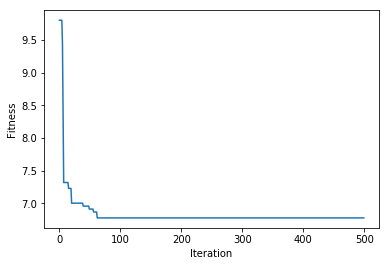
\includegraphics[height=2.5in]{10MSTA1.png}}
\caption{SDS 1 on 10 Vertices MST
processes } \label{SDS1 G10}
\end{figure}

\begin{table}
\centering
\caption{10 Verticex MST}
\begin{tabular}{l|lllll}
	   & Best    & Worst    &   Mean  & Median & SD \\ \hline
SDS 1  & 8.7127 & 28.6777 & 15.5151 & 16.5061 & 5.8357 \\
SDS 2  & 8.7127 & 26.3134 & 14.8274 & 15.3896 & 5.5623	\\
SDS 3  & 8.7127 & 25.5691 & 14.8404	& 14.7548 & 5.5969 \\
Kruskal &8.7127 & 33.4938 & 		&  & \\
\end{tabular}
\end{table}

\begin{table}
\centering
\caption{20 Verticex MST}
\begin{tabular}{l|lllll}
	   & Best    & Worst    &   Mean  & Median & SD \\ \hline
SDS 1  & 6.2154 & 26.6922 & 13.8273 & 15.9216	 & 6.6259	 \\
SDS 2  & 6.2154 & 27.0327 & 13.6328	 & 14.4529	 & 6.8562	\\
SDS 3  & 6.2154 & 28.7356	 & 14.5261	& 17.0498	 & 6.8479 \\
Kruskal &6.2154 & 33.2481 & 		&  & \\
\end{tabular}
\end{table}

\begin{table}
\centering
\caption{30 Verticex MST}
\begin{tabular}{l|lllll}
	   & Best    & Worst    &   Mean  & Median & SD \\ \hline
SDS 1  & 1.5844	&  8.2090 & 4.3842  & 5.8027 & 2.5179 \\
SDS 2  & 1.5212 & 8.2174 & 4.2071 & 5.6152 & 2.5304 \\
SDS 3  & 1.5212 & 7.90981 & 4.0656	& 3.5756 & 2.4923 \\
Kruskal &1.5212 & 11.6982 & 		&  & \\
\end{tabular}
\end{table}

\begin{table}
\centering
\caption{40 Verticex MST}
\begin{tabular}{l|lllll}
	 	  & Best    & Worst    &   Mean  & Median & SD \\ \hline
SDS 1 & 1.2256	 & 5.6444  & 3.0480 & 1.4553 & 1.7944 \\
SDS 2 & 1.1046	 & 5.6780	& 3.1405 & 4.4635 & 1.8890 \\	
SDS 3 & 1.1046	 & 5.7676	& 3.1981 & 4.3862 & 1.8882 \\	
Krushkal      & 1.0598	 & 8.4946 \\
\end{tabular}
\end{table}

\begin{table}
\centering
\caption{50 Verticex MST}
\begin{tabular}{l|lllll}
	   & Best    & Worst    &   Mean  & Median & SD \\ \hline
SDS 1 &  1.0403 & 4.5785	& 2.5420	& 3.4940	& 1.3917 \\
SDS 2 & 0.8923	 & 4.5699	& 2.3721	& 1.0254	& 1.4800 \\	
SDS 3 & 0.8923	 & 4.5358	& 2.4153	& 3.3701	& 1.4682 \\	
Krushkal &	0.7984 &	7.0051 \\
\end{tabular}
\end{table}



\section{Discussion}

The table MST 10 has shown that all three implementations of SDS are able to reach the optimal solution and return a MST. It appears that SDS 3 has the largest standard deviation which means that is has the higher exploration rate of the three algorithms. An effect of this larger exploration rate appears to be that it is more like to find bad results. Another observation is that the only algorithm whose worst result is within 2 standard deviations was the 3rd approach. This is rather significant as there is around a 2\%\ chance per agent to vary this far into bad solutions. The cause is of this is likely the population size as 200 agents is a fair amount.

In the second table the algorithm containing the worst agent has change from SDS 1 to SDS 3. This is interesting as in MST the result was the other way around. This is probably due to the stochastic nature of the algorithm. It should be noted that none of the agents are outside of a standard deviation of two for this test. There does not appear to be any trends in terms of worst, mean, median and standard deviation so far.

MST 30 is where things become more interesting as one of the SDS algorithms failed to converge on the optimal spanning tree. It comes as no surprise that SDS 1 has failed; it consistently has the worst performance of the three algorithms as it is always the last to converge on a solution. In contrast to this both SDS 2 and 3 have reached the solution. Based on the median and standard deviation for this benchmark it would appear that SDS 3 has the highest exploitation out of these approaches. 

The graphs presented show an interesting phenomenon in which both SDS 2 and SDS 3 are converging on the optimal solution in the first iterations. This cause of this is unknown and further research should be conducted as this could potentially be the fastest swarm intelligent meta-heuristic. If this property holds with a lower number of agents I could mean that SDS has the potential to be one of the fastest algorithms for finding spanning trees. As for SDS 1 the convergence appears to be similar to the GA for MST.
One last note that is not related to SDS but more so randomly generated complete graphs is the fact that the larger the graph becomes the smaller the MSP. This trend is appears throughout all or the data presented. 



\section{Evaluation}

The implementation of SDS for MST was success and has led to some interesting discoveries. The programme has fulfilled all requirements due to the use of test driven development. However this has come with a great deal of problems mostly due to the design of the program. Sub optimal methods have been used in the implementation of the SDS algorithm. This is the cause of the largest issue of this project, the time taken for the program to run. This has been a difficult learning curve and has shown the true importance of optimising the time complexity of each algorithm in addition to selecting the correct data structures when implementing these algorithms.


\section{Conclusion}

The aim of this project was to determine whether the SDS algorithm would be able to converge on the MST of any given graph. Overall this project was successful as it has proven that multiple variations of SDS are capable of producing MSTs from a graph. From the research produced from the implementation of SDS an interesting scenario consistently occurred where SDS 2 and 3 would converge within the first iteration. More research is required to discover the cause of these convergence rates as it could potentially lead to faster solutions for the MST problem.


\section{Future Deveolpment}

One of the major issues in this project is the time it takes to complete a full cycle of SDS on larger graph sizes. For example with the parameters of 200 agents and 500 iterations on a complete graph of 100 nodes the time taken to complete SDS became around 10 minutes. This became exponentially worse for a complete graph of 200 nodes as the time grew to over an hour.
This issue arose from the time complexity of Kruskal’s and Stochastic Kruskal’s using the DFS algorithm to detect loops. As the DFS algorithm takes place within an iteration of all edge the time complexity rises to {$O (E2)$}. To fix this a dis-jointed data structure will need to be created to replace the DFS algorithm. This will drastically increase the performance as the methods in that will be used from this data structure operate in constant time {$O (1)$}. In addition to this an implicit implementation for the graph would also provide a minor improvement in speed.
Another solution would be to implement and alternative hypothesis the agent class. An example of this would be to generate a pürfer numbers much like the GA approach. This way each hypothesis would represent a unique spanning tree for the graph which would remove the need to generate random graphs and check for spanning tree or cycles.
Upon completing these update this project can be used as the gateway into the NP-hard MST problems which are known as the degree constrained MST and capacitated MST.


\bibliography{references_NC}

\section{Appendix}

\end{document}
